\documentclass[a4paper,12pt]{article}
%%% Работа с русским языком % для pdfLatex
\usepackage{cmap}					% поиск в~PDF
\usepackage{mathtext} 				% русские буквы в~фомулах
\usepackage[T2A]{fontenc}			% кодировка
\usepackage[utf8]{inputenc}			% кодировка исходного текста
\usepackage[english,russian]{babel}	% локализация и переносы
\usepackage{indentfirst} 			% отступ 1 абзаца
\usepackage{gensymb}				% мат символы?

%%% Работа с русским языком % для XeLatex
%\usepackage[english,russian]{babel}   %% загружает пакет многоязыковой вёрстки
%\usepackage{fontspec}      %% подготавливает загрузку шрифтов Open Type, True Type и др.
%\defaultfontfeatures{Ligatures={TeX},Renderer=Basic}  %% свойства шрифтов по умолчанию
%\setmainfont[Ligatures={TeX,Historic}]{Times New Roman} %% задаёт основной шрифт документа
%\setsansfont{Comic Sans MS}                    %% задаёт шрифт без засечек
%\setmonofont{Courier New}
%\usepackage{indentfirst}
%\frenchspacing

%%% Дополнительная работа с математикой
\usepackage{amsfonts,amssymb,amsthm,mathtools}
\usepackage{amsmath}
\usepackage{icomma} % "Умная" запятая: $0,2$ --- число, $0, 2$ --- перечисление
\usepackage{upgreek}

%% Номера формул
%\mathtoolsset{showonlyrefs=true} % Показывать номера только у тех формул, на которые есть \eqref{} в~тексте.

%%% Страница
\usepackage{extsizes} % Возможность сделать 14-й шрифт

%% Шрифты
\usepackage{euscript}	 % Шрифт Евклид
\usepackage{mathrsfs} % Красивый матшрифт

%% Свои команды
\DeclareMathOperator{\sgn}{\mathop{sgn}} % создание новой конанды \sgn (типо как \sin)
\DeclareMathOperator{\rg}{\mathop{rg}}
\DeclareMathOperator{\Rg}{\mathop{Rg}}
\DeclareMathOperator{\im}{\mathop{Im}}
%\DeclareMathOperator{\dim}{\mathop{dim}}
\usepackage{csquotes} % ещё одна штука для цитат
\newcommand{\pd}[2]{\ensuremath{\cfrac{\partial #1}{\partial #2}}} % частная производная
\newcommand{\abs}[1]{\ensuremath{\left|#1\right|}} % модуль
\renewcommand{\phi}{\ensuremath{\varphi}} % греческая фи
\newcommand{\pogk}[1]{\!\left(\cfrac{\sigma_{#1}}{#1}\right)^{\!\!\!2}\!} % для погрешностей

% Ссылки
\usepackage{color} % подключить пакет color
% выбрать цвета
\definecolor{BlueGreen}{RGB}{49,152,255}
\definecolor{Violet}{RGB}{120,80,120}
% назначить цвета при подключении hyperref
\usepackage[unicode, colorlinks, urlcolor=blue, linkcolor=blue, pagecolor=blue, citecolor=blue]{hyperref} %синие ссылки
%\usepackage[unicode, colorlinks, urlcolor=black, linkcolor=black, pagecolor=black, citecolor=black]{hyperref} % для печати (отключить верхний!)


%% Перенос знаков в~формулах (по Львовскому)
\newcommand*{\hm}[1]{#1\nobreak\discretionary{}
	{\hbox{$\mathsurround=0pt #1$}}{}}

%%% Работа с картинками
\usepackage{graphicx}  % Для вставки рисунков
\graphicspath{{images/}{images2/}}  % папки с картинками
\setlength\fboxsep{3pt} % Отступ рамки \fbox{} от рисунка
\setlength\fboxrule{1pt} % Толщина линий рамки \fbox{}
\usepackage{wrapfig} % Обтекание рисунков и таблиц текстом
\usepackage{multicol}

%%% Работа с таблицами
\usepackage{array,tabularx,tabulary,booktabs} % Дополнительная работа с таблицами
\usepackage{longtable}  % Длинные таблицы
\usepackage{multirow} % Слияние строк в~таблице
\usepackage{caption}
\captionsetup{labelsep=period, labelfont=bf}

%%% Оформление
\usepackage{indentfirst} % Красная строка
%\setlength{\parskip}{0.3cm} % отступы между абзацами
%%% Название разделов
\usepackage{titlesec}
\titlelabel{\thetitle.\quad}
\renewcommand{\figurename}{\textbf{Рис.}}		%Чтобы вместо figure под рисунками писал "рис"
\renewcommand{\tablename}{\textbf{Таблица}}		%Чтобы вместо table над таблицами писал Таблица
\usepackage{enumitem}
\setlist{nolistsep}
\usepackage{verbatim}

%%% Теоремы
\theoremstyle{plain} % Это стиль по умолчанию, его можно не переопределять.
\newtheorem{theorem}{Теорема}[section]
\newtheorem{proposition}[theorem]{Утверждение}
\newtheorem{predlog}{Предложение}[section]
\newtheorem{lemma}{Лемма}[section]

\theoremstyle{definition} % "Определение"
\newtheorem{definition}{Определение}[section]
\newtheorem{corollary}{Следствие}[theorem]
\newtheorem{problem}{Задача}[section]

\theoremstyle{remark} % "Примечание"
\newtheorem*{nonum}{Решение}
\newtheorem{zamech}{Замечание}[theorem]

%%% Правильные мат. символы для русского языка
\renewcommand{\epsilon}{\ensuremath{\varepsilon}}
\renewcommand{\phi}{\ensuremath{\varphi}}
\renewcommand{\kappa}{\ensuremath{\varkappa}}
\renewcommand{\le}{\ensuremath{\leqslant}}
\renewcommand{\leq}{\ensuremath{\leqslant}}
\renewcommand{\ge}{\ensuremath{\geqslant}}
\renewcommand{\geq}{\ensuremath{\geqslant}}
\renewcommand{\emptyset}{\varnothing}

%%% Для лекций по инфе
\usepackage{alltt}
\newcounter{infa}[section]
\newcounter{num}
\definecolor{infa}{rgb}{0, 0.2, 0.89}
\definecolor{infa1}{rgb}{0, 0.3, 1}
\definecolor{grey}{rgb}{0.5, 0.5, 0.5}
\newcommand{\tab}{\ \ \ }
\newcommand{\com}[1]{{\color{grey}\##1}}
\newcommand{\num}{\addtocounter{num}{1}\arabic{num}\tab}
\newcommand{\defi}{{\color{infa}def}}
\newcommand{\ini}{{\color{infa}in}}
\newcommand{\rangei}{{\color{infa}range}}
\newcommand{\fori}{{\color{infa}for}}
\newcommand{\ifi}{{\color{infa}if}}
\newcommand{\elsei}{{\color{infa}else}}
\newcommand{\printi}{{\color{infa1}print}}
\newcommand{\maxi}{{\color{infa}max}}
\newcommand{\classi}{{\color{infa}class}}
\newcommand{\returni}{{\color{infa}return}}
\newcommand{\elifi}{{\color{infa}elif}}
\newenvironment{infa}[1]{
	
	\vspace{0.5cm}
	\addtocounter{infa}{1}%
	\noindent{\large \textbf{Программа №\thesection.\arabic{infa}}}\textbf{<<#1>>}%
	\begin{alltt}%
	}{\end{alltt}
	\setcounter{num}{0}
	\vspace{0.1cm}}
%Пример кода:
%\begin{infa}{Поразрядная сортировка}
%	\ \num \defi count_sort(a):\tab \com{определяет нашу функцию}
%	\ \num \tab m = \maxi(a)+1
%	\ \num \tab q = [0]*m
%	\ \num \tab \fori x \ini a:
%	\ \num \tab \tab q[x] += 1
%	\ \num \tab pos = 0
%	\ \num \tab \fori x \ini q:
%	\ \num \tab \tab \fori i \ini \rangei(q[x]):
%	\ \num \tab \tab \tab a[pos] = x
%	\num \tab \tab \tab pos += 1
%\end{infa}

\renewcommand{\baselinestretch}{1.3}

\title{vopr}
\author{Георгий Демьянов}
\date{today}
\usepackage[left=1.27cm,right=1.27cm,top=1.27cm,bottom=2cm]{geometry}

\begin{document}
\begin{center}
	\textbf{Вопрос по выбору}
\end{center}	

Пусть есть поршень, который находится в термостате с температурой $T_0$ и с бесконечной теплоемкостью.

Поставим вопрос: \textbf{возможно ли построить тепловой двигатель, имея один источник тепла?}
\begin{figure}[h!]
	\centering
	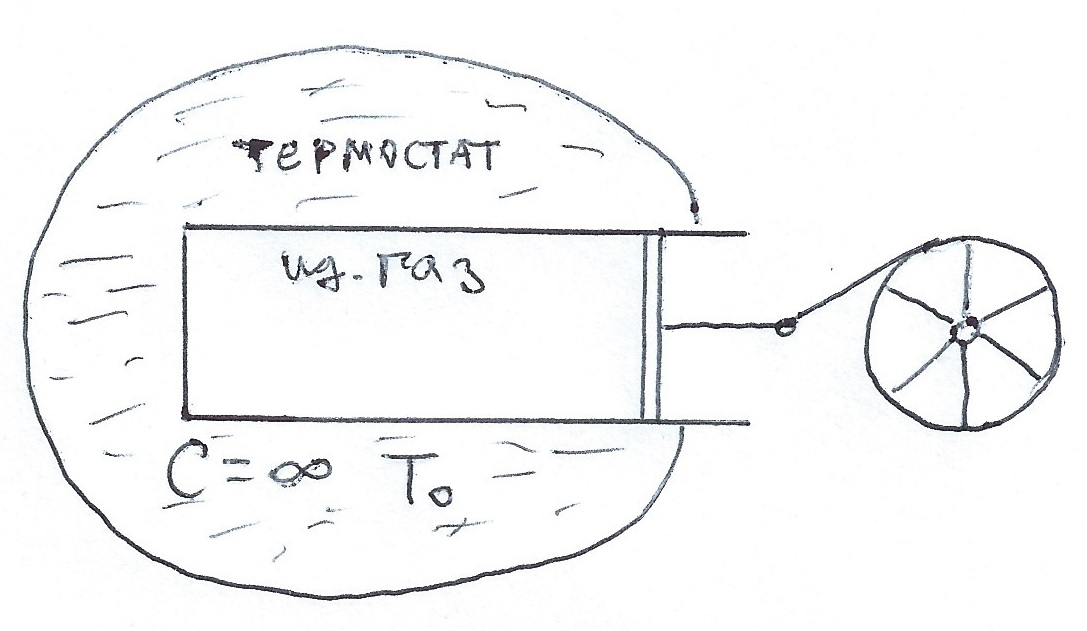
\includegraphics[width=0.3\linewidth]{ris1}
	\caption{Поршень в термостате}
	\label{fig:ust}
\end{figure}

Тогда на $PV$--диаграмме можно изобразить только изотерму.
\begin{figure}[h!]
	\centering
	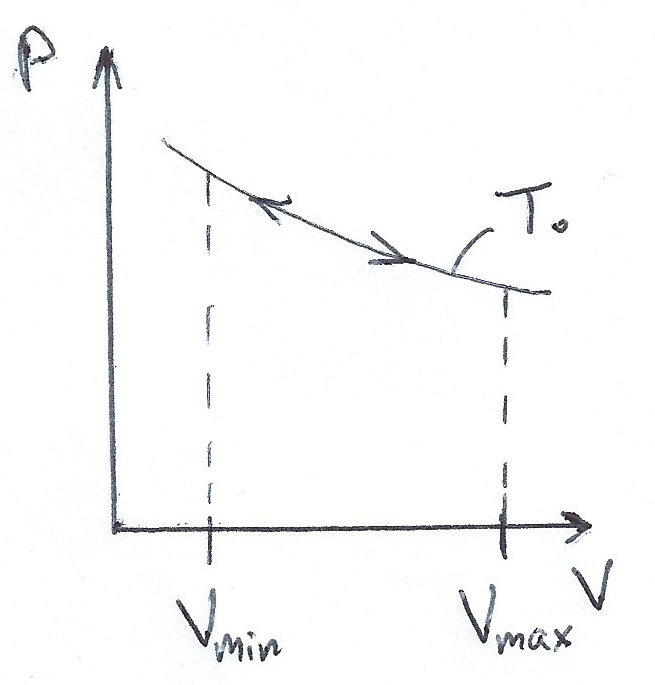
\includegraphics[width=0.25\linewidth]{ris2}
	\caption{$PV$--диаграмма}
	\label{fig:ust}
\end{figure}
Если мы будем двигаться вдоль по изотерме <<вперед--назад>>, то полезная работа будет равна нулю, т.е. смысла в такой машине нет.

Что же можно сделать еще? Если наш поршень находится в адиабатической оболочке, то мы можем <<бегать>> по адиабате, для чего нужно совершать достаточно быстрые движения поршнем.
\begin{figure}[h!]
	\centering
	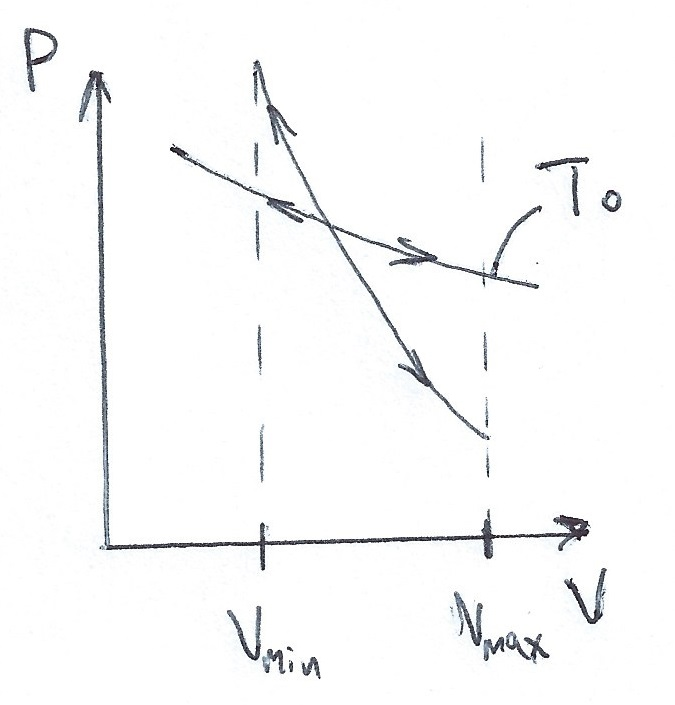
\includegraphics[width=0.25\linewidth]{ris3}
	\caption{$PV$--диаграмма}
	\label{fig:ust}
\end{figure}
В нашем же случае попытаемся построить такой процесс, который был бы чем-то средним между изотермой и адиабатой. Тогда нужно двигать поршень не бесконечно медленно (т.е. <<бегать>> не по изотерме), а немного быстрее, но не так быстро, чтобы попасть на адиабату. Тогда будет существовать теплообмен между идеальным газом и термостатом. При этом, будем утверждать, что газ в каждый момент времени будет достаточно отрелаксированным.

Для того, чтобы построить такой процесс, найдем зависимость $\Delta P = \Delta P(Q, \Delta V)$.

Запишем первое начало термодинамики в приращениях:
\begin{equation}
C_V \Delta T = Q - P\Delta V,
\end{equation}
где $C_V$ --- теплоемкость газа при постоянном объеме, $\Delta T$ --- малые изменения температуры, $\Delta V$ --- малые изменения объема, $Q$ --- тепло, $P$ --- давление газа.

Запишем уравнение состояния идеального газа для 1 моля в приращениях:
\begin{equation}
P\Delta V+V\Delta P = R\Delta T.
\end{equation}

Решая систему из этих уравнений, получим:
\begin{equation}
\boxed{
\Delta P = \cfrac{R}{VC_V}\,Q-\cfrac{\gamma P}{V}\,\Delta V},
\label{main}
\end{equation}
где $\gamma$ --- показатель адиабаты.

Т.о. мы получили зависимость изменения давления идеального газа, который совершает работу $P\Delta V$ и обменивается теплом $Q$ с термостатом. Заметим, что при $Q=0$ получаем $\Delta P_{\text{ад}} = -\frac{\gamma P}{V}\,\Delta V$ --- изменение давления в адиабатическом процессе. Тогда запишем уравнение \eqref{main} в кратком виде:
\begin{equation}
\boxed{
\Delta P = \cfrac{R}{VC_V}\,Q+\Delta P_{\text{ад}}}.
\label{main2}
\end{equation}

Построим $PV$--диаграммы (рис. \ref{fig:res}).\\
\begin{figure}[h!]
	\centering
	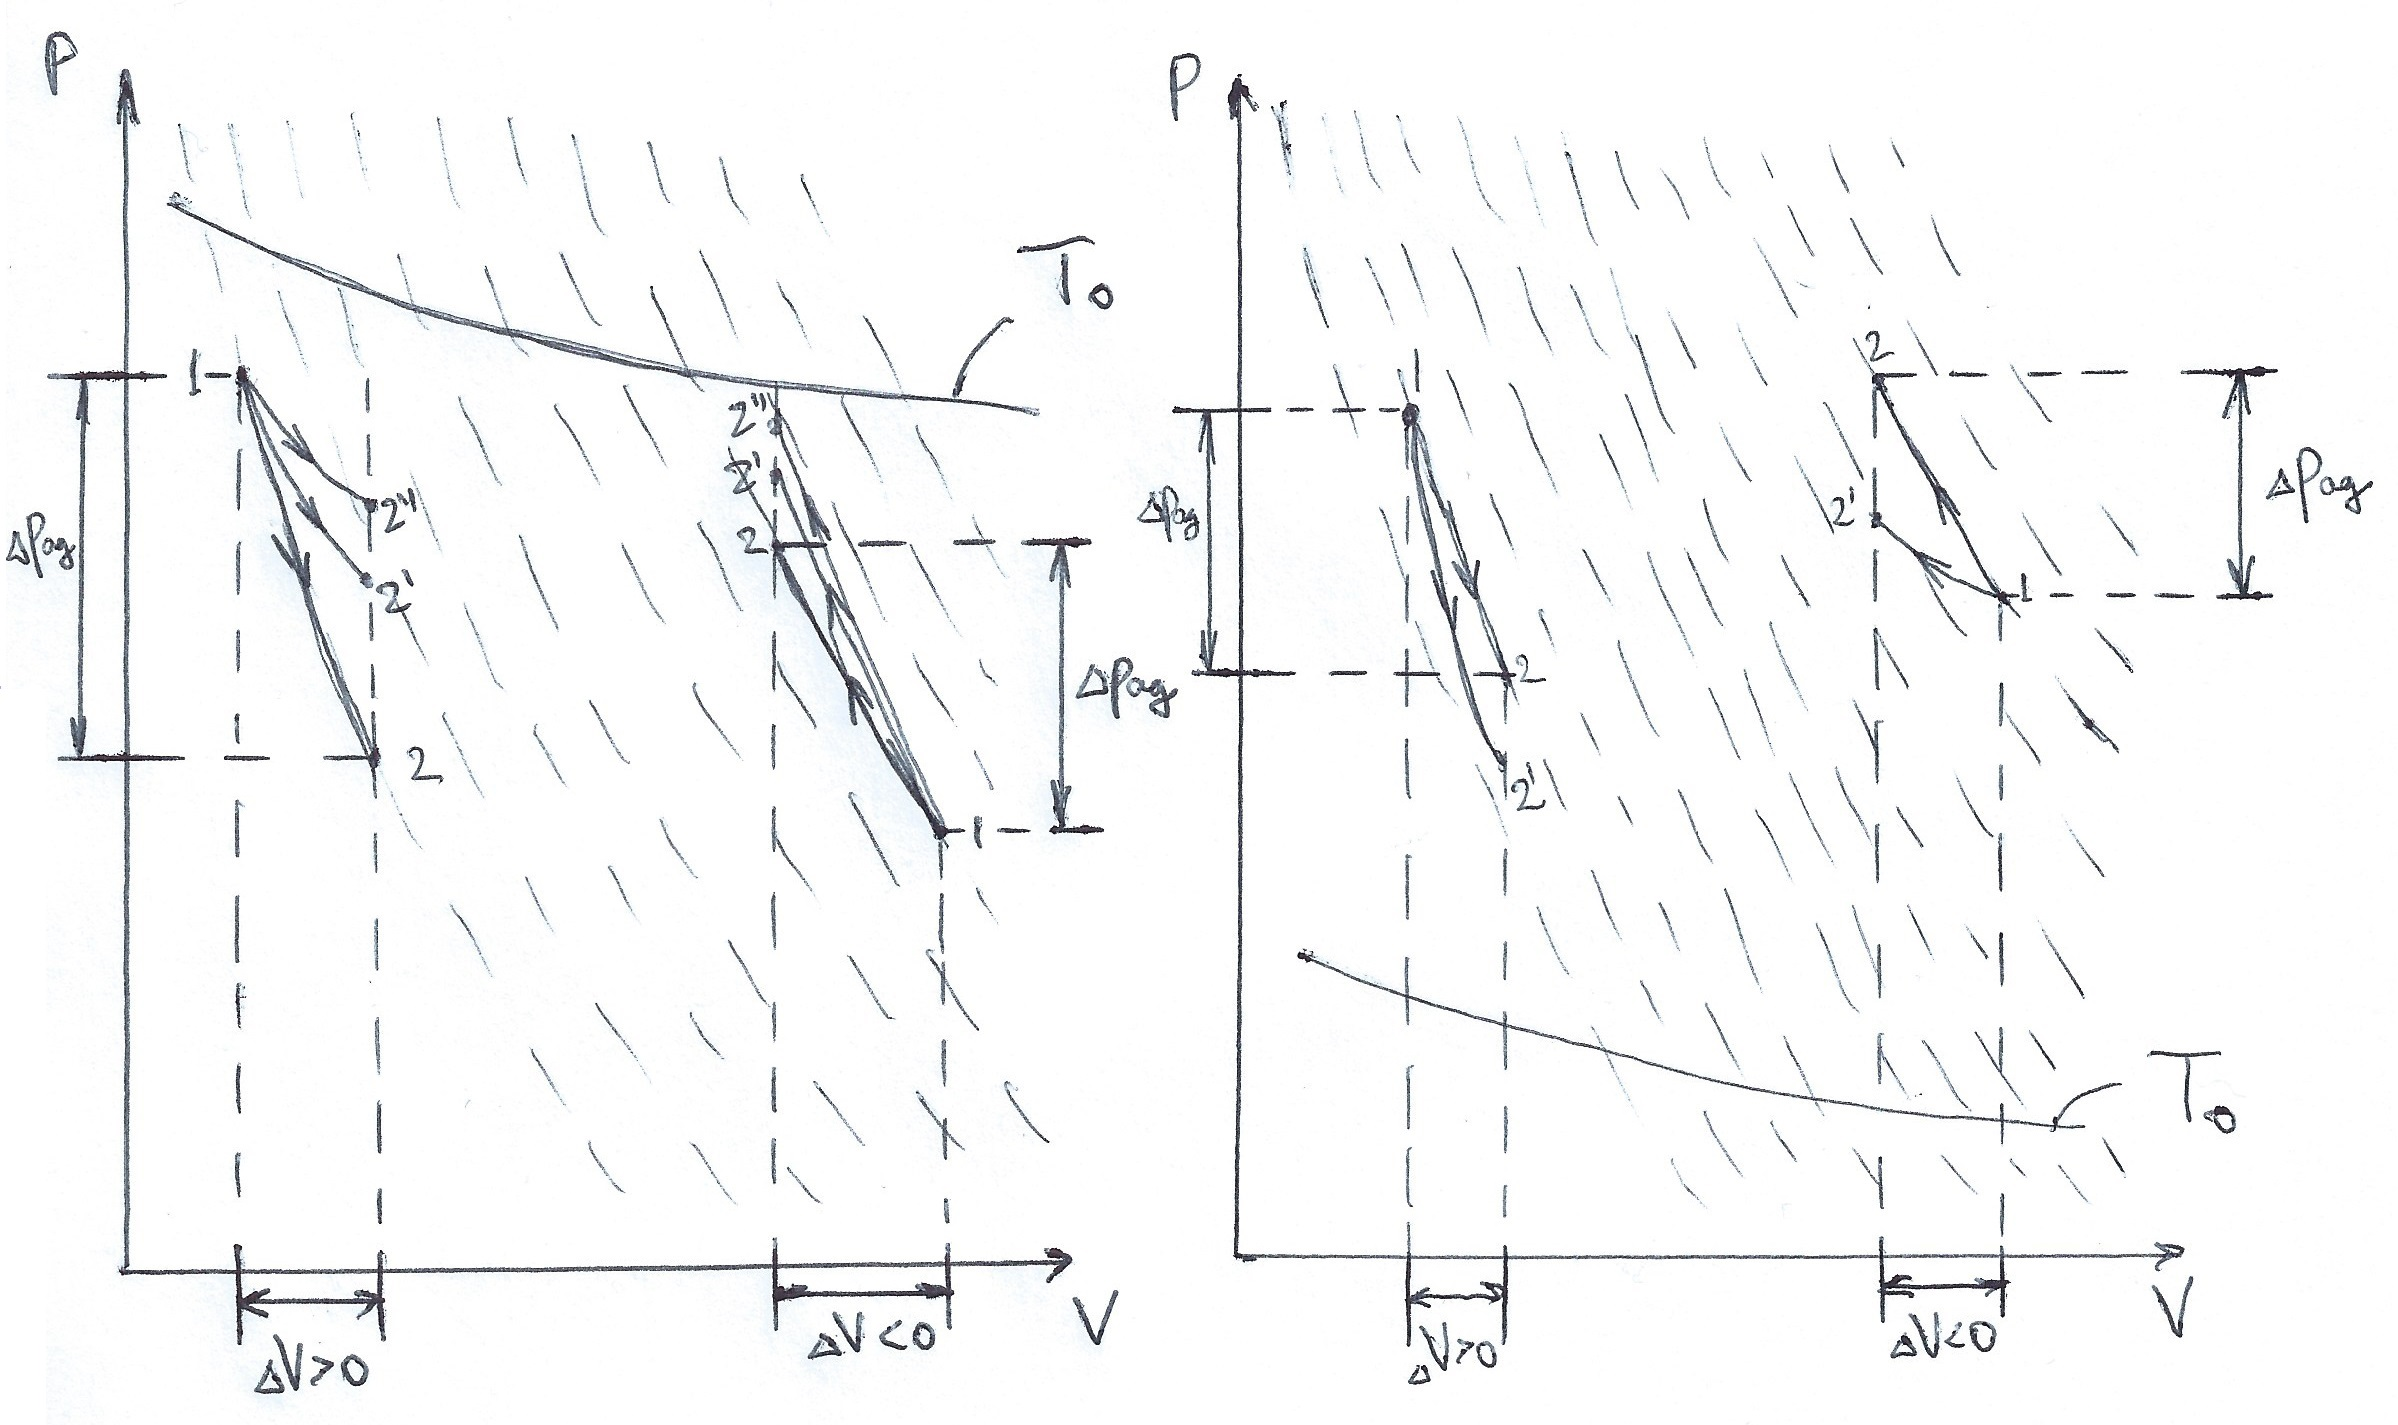
\includegraphics[width=0.9\linewidth]{ris4}
	\caption{$PV$--диаграмма}
	\label{fig:res}
\end{figure}
Рассмотрим два случая:\\
I. $Q>0$, т.е. $T_{\text{г}} < T_0$ (слева);\\
II. $Q<0$, т.е. $T_{\text{г}} > T_0$ (справа).\\
На диаграммах пунктиром изображено семейство адиабат, изотерма с температурой $T_0$. 

\begin{enumerate}
	\item[I.] \begin{enumerate}
		\item[1)] Рассмотрим расширение газа по адиабате ($1\rightarrow 2$). $Q>0$, $\Delta P_{\text{ад}}<0$, отсюда в соответствии с формулой \eqref{main2} $\abs{\Delta P}<\abs{\Delta P_{\text{ад}}}$. Таким образом, мы будем наблюдать <<загибание процесса>> ($1\rightarrow 2'$ или $1\rightarrow 2''$).
		\item[2)] Рассмотрим сжатие газа по адиабате ($1\rightarrow 2$). $Q>0$, $\Delta P_{\text{ад}}>0$, отсюда в соответствии с формулой \eqref{main2} $\abs{\Delta P}>\abs{\Delta P_{\text{ад}}}$. Таким образом, наклон графика процесса выглядит <<круче>>, чем в адиабатическом процессе ($1\rightarrow 2'$ или $1\rightarrow 2''$).
	\end{enumerate}
	Можно наблюдать, что добавка теплоты $Q$ приближает процесс к изотерме $T_0$.
	\item[II.] \begin{enumerate}
		\item[1)] Рассмотрим расширение газа по адиабате ($1\rightarrow 2$). $Q<0$, $\Delta P_{\text{ад}}<0$, отсюда в соответствии с формулой \eqref{main2} $\abs{\Delta P}>\abs{\Delta P_{\text{ад}}}$. Таким образом, процесс <<будет идти>> стремительнее ($1\rightarrow 2'$).
		\item[2)] Рассмотрим сжатие газа по адиабате ($1\rightarrow 2$). $Q<0$, $\Delta P_{\text{ад}}>0$, отсюда в соответствии с формулой \eqref{main2} $\abs{\Delta P}<\abs{\Delta P_{\text{ад}}}$. Таким образом, процесс <<будет идти>> менее <<круто>> ($1\rightarrow 2'$).
	\end{enumerate}
\end{enumerate}
В итоге получаем, что все процессы стремятся к изотерме $T_0$.

А теперь попробуем построить круговой процесс.
\begin{figure}[h!]
	\centering
	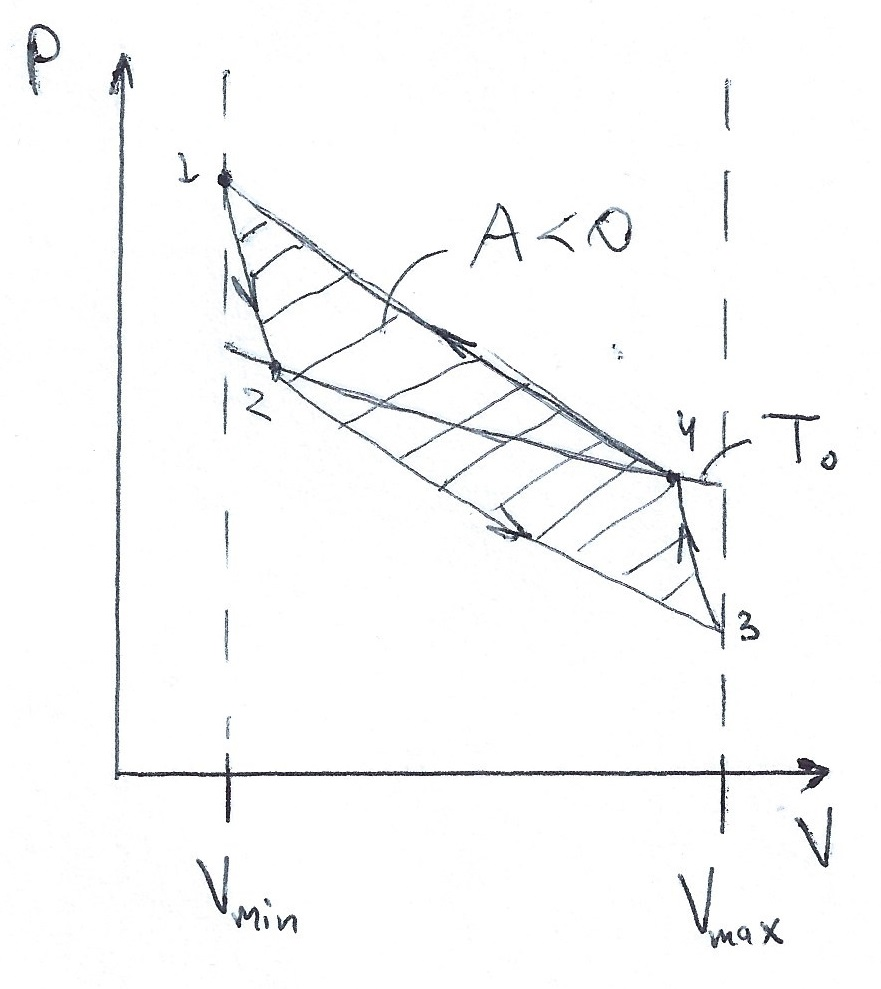
\includegraphics[width=0.3\linewidth]{ris5}
	\caption{Круговой процесс}
	\label{fig:ust}
\end{figure}

Таким образом, \textit{мы получили ход против часовой стрелки} ($A<0$), причем этот \textit{процесс необратим}. Обратного хода быть не может, т.к. есть теплообмен газа и резервуара.

Заметим, что чем медленнее будем двигаться, там <<уже>> будет картинка, т.е. мы приближаемся к изотерме. Чем быстрее будем двигаться, тем картинка <<шире>>, т.е. процесс приближается к адиабатическому.

Мы получили утилизатор работы.

\textbf{Вывод:} \textit{имея один тепловой резервуар, нельзя построить тепловую машину, но можно построить утилизатор работы.}

Отсюда легко получить \textbf{неравенство Клаузиуса}:

Пусть мы имеем один тепловой резервуар. Газ можно перевести из состояния 1 в состояние 2 двумя способами: обратимым и необратимым.
\begin{figure}[h!]
	\centering
	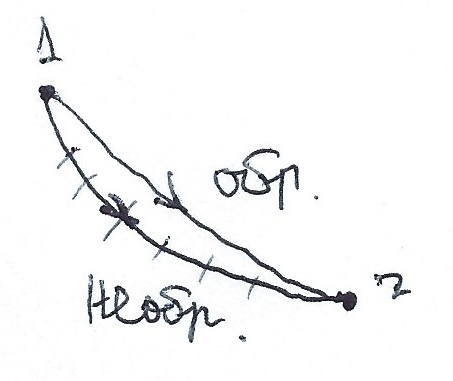
\includegraphics[width=0.2\linewidth]{ris6}
	%\caption{Круговой процесс}
	\label{fig:ust}
\end{figure}

\begin{center}
$
\delta Q^{\text{ноб}}=dU+\delta A^{\text{ноб}}$\\
$\delta Q^{\text{об}}=dU+\delta A^{\text{об}}
$
\end{center}
Из этого можно получить круговой процесс путем обращения обратимого процесса. Тогда:
\begin{center}
$\delta Q = \delta Q^{\text{ноб}}-\delta Q^{\text{об}} = \delta A^{\text{ноб}}-\delta A^{\text{об}} \leq 0$ --- по доказанному\\
$\delta Q^{\text{ноб}}\leq\delta Q^{\text{об}} = TdS$\\
$dS\geq \cfrac{\delta Q^{\text{ноб}}}{T}$
\vspace{-0.5cm}
$$0=\oint\limits dS\geq \oint{\cfrac{\delta Q^{\text{ноб}}}{T}}$$
$$\boxed{\oint{\cfrac{\delta Q^{\text{ноб}}}{T}}\leq0}\text{ --- \textbf{неравенство Клаузиуса.}}$$
\end{center}

Отсюда следует, что в необратимых адиабатически--изолированных процессах энтропия не убывает --- \textbf{закон возрастания энтропии}:
$$
dS\geq \cfrac{\delta Q^{\text{ноб}}}{T}=0 \Rightarrow dS\geq 0.
$$








\begin{center}
	\vfill \emph{{\small Г. С. Демьянов, 642 группа, 2017 г.}}
\end{center}
\end{document}